\section{Simulieren}

\subsection{Die Entstehung von Galaxien}
``Eine Galaxie ist eine durch Gravitation gebundene große Ansammlung von
Sternen, Planetensystemen, Gasnebeln und sonstigen Stellaren Objekten.``
\footnote{\url{https://de.wikipedia.org/wiki/Galaxie}}

Demnach ist es relativ Einfach eine Galaxie zu generieren: es werden einfach
ganz viele Objekte in einen Raum geworfen. Das reicht jedoch nicht um die
Objekte als Galaxie definieren zu können, da sie nicht ``durch Gravitation
gebunden`` sind.

Um dies zu tun muss die Kraft zwischen allen Objekten in der Galaxie berechnet
werden um damit die Position der jeweiligen Objekte nach einer bestimmten Zeit
bestimmen zu können.

Dies reicht jedoch auch nicht um eine ``stabile`` Galaxie zu generieren:
berechnet man nur die Kräfte die auf ruhende Objekte in einem Reibungsfreiem Raum
wirken, würden alle Objekte zum Massenmittelpunkt gezogen werden und die Galaxie
würde somit implodieren. Es ist also nötig auf die Sterne in der Galaxie
Anfangs Kräfte zu wirken.  Diese Kräfte sind durch die Rotation der Galaxie um
den Massenmittelpunkt der Galaxie definiert, man rotiert also die Galaxie und
gleicht durch die Zentripetalkraft, die Kraft die Alle Sterne Richtung
Massenmittelpunkt zieht aus. Rotiert man die Galaxie jedoch zu schnell,
explodiert sie Förmlich, da die Sterne nicht mehr zusammengehalten werden und
die Fliehkraft sie einfach auseinanderzieht.

\subsection{Berechnung der Beschleunigungen}
Um die Beschleunigung die auf einen Stern wirkt zu berechnen wird folgendes
berechnet:

\begin{equation} \label{eq:beschleunigung}
    a = G \cdot \frac{\Delta{M_2}}{\Delta{r}^2}
\end{equation}

\( G \) steht hier für die Universelle Gravitationskraft, \( \Delta M \) für die
Masse des Objektes das Umkreist wird und \( \Delta r \) für die Entfernung zum
Mittelpunkt des Objektes das umkreist wird.
Problem ist, dass kein Objekt umkreist wird sondern eine große Anzahl an Sternen.
Es ist also nicht möglich mithilfe von herkömmlichen Methoden die Beschleunigung
die auf einen Stern wirkt zu berechnen.

TODO: und jetzt?

\subsubsection{Die Kraft als Vektor}
Um die Kraft als Vektor darzustellen, muss die Formel \ref{eq:beschleunigung}
mithilfe von Vektoren wiefolgt neu aufgestellt werden:

\begin{equation} \vec{F}_{12} = \underbrace{-G \frac{m_1 m_2}{|r_{12}|^2}}_{Scalar}
\cdot \underbrace{\frac{r_2 - r_1}{|r_2 - r_1|}}_{Vector} \end{equation}

Die Summe der Kräfte die auf einen Stern wirken ist somit die Summe aller
Kräfte die zwischen dem jeweiligen Stern \( a \) und allen anderen Sternen
wirken:

\begin{equation} F_{a} = \sum_{i=0}^{n-1} F_{ai} \end{equation}

\subsubsection{Berechnung der Umlaufgeschwindigkeit}
Die Umlaufgeschwindigkeit kann berechnet werden, indem die Kraft die die Sterne
in die Mitte der Galaxie zieht \( \left( F = G \cdot \frac{m \cdot M}{r^2}
\right) \) mit der Zentripetalkraft \( \left( F_z = \frac{m \cdot v^2}{r}
\right)\) gleichgesetzt wird:

\begin{equation}
v = \sqrt{\frac{G \cdot M_E}{r}}
\end{equation}

\( M_E \) steht dabei für die Masse der Erde, \( G \) für die
Gravitationskonstante und \( r \) für den Bahn Radius.  Da wir jedoch nicht in
der Erdumlaufbahn, sondern in einer Galaxien Umlaufbahn hantieren, können wir
nicht die Masse der Erde nutzen. Wir müssen daher eine andere Möglichkeit
nutzen, die Größe der Masse, die den Stern in Richtung Massenmittelpunkt zieht zu
berechnen.

\subsubsection{Ellipsen und die Geschwindigkeit der Sterne}
Da die Sterne nicht auf perfekten Kreisbahnen um den Mittelpunkt der Galaxie
fliegen muss in betracht gezogen werden wie die Sterne auf Elliptischen Bahnen
orbitieren.  Wichtigt ist dabei die Geschwindigkeit, diese muss zwischen der
ersten Kosmischen Geschwindigkeit \( v_k \) und der zweiten Kosmischen
Geschwindigkeit \( v_P \) liegen. Die beiden Kosmischen Geschwindigkeiten sind
folgendermaßen definiert:

\begin{equation}
v_{k1} = \sqrt{\frac{GM}{r}}
\end{equation}
\begin{equation}
v_{k2} = \sqrt{\frac{2GM}{r}}
\end{equation}

Die Tatsache das die Sterne auf Elliptischen Bahnen unterwegs sind ist für die
Berechnung irrelevant, da eh für jeden Zeitschritt \( t \) eine neue Kraft
berechnet wird aus der eine Beschleunigung berechnet wird die wiederum die neue
Position des Sternes ergibt.  Hält man die Geschwindigkeit der Sterne somit im
Intervall \( (v_{k1} ; v_{k2}) \), dann ergibt sich (in der Theorie) von
alleine eine elliptische Bahn.

\subsection{Entwicklung der nötigen Software}
Die Software ist komplett in Golang geschrieben was die Nutzung von mehreren
Threads mithilfe von Go-Methoden stark vereinfacht. Um den Barnes-Hut
Algorithmus anzuwenden muss die Galaxie in einen Octree unterteilt werden.
Dabei wird eine Zelle definiert die alle Sterne beinhaltet welche anschließen
solange unterteilt, bis eine der drei End Bedingungen eintrifft.

\subsubsection{Zu lösende Probleme}
Ein Problem das auftritt wenn die Kräfte zwischen allen Sternen berechnet
werden ist, dass der Rechenaufwand \( O(n \cdot n-1) \approx O(n^2) \) beträgt.

Es kommt zu Problemen, wenn der mittlere Fehler, der bei der Berechnung der Kraft
entsteht größer als die wirkende Kraft wird. Dies passiert unter anderem dann,
wenn der Abstand zwischen den Sternen so groß wird, das die wirkende Kraft so gering ist
das sie mithilfe von Computern nicht mehr sinnvoll dargestellt wird.
Statt nun mit Rundungsfehlern zu rechnen, können diese Sterne, die sehr weit entfernt vom
Stern dessen Kräfte berechnet werden sollen, einfach nicht mehr beachtet werden,
da sie nicht sinnvoll beitragen.
Um dieses Problem zu lösen wird der Barnes-Hut Algorithmus verwenden. Dieser Algorithmus
unterteilt einen Bereich in variabel große Zellen und mindert die Laufzeit von \( O(n^2) \) auf
\( O(n \log(n) \).

\subsubsection{Generierung von Quadtrees und die Nutzung des Barnes-Hut
Algorithmus}

Um nun einen Quadtree (einen k-nären Baum mit jeweils vier Kindern) zu
generieren die die komplette Galaxie umfasst, muss erstmal definiert werden wie
groß die Galaxie überhaupt ist. Dazu werden, falls bereits Sterne vorliegen,
die jeweiligen Extrempunkte (minimales x, minimales y, maximales x und
maximales y) bestimmt und die Wurzel Zelle mithilfe diese Werte entsprechend
skaliert.  Falls jedoch noch nicht bekannt ist wie groß die Galaxie sein wird,
muss abgeschätzt werden wir groß sie werden könnte, d.h.: es wird bei der
Generierung geschaut in was für einem Bereich die Sterne Generiert werden. 

\begin{equation}
    \text{Wurzel Knoten} = (0, 0), \text{Breite}=b
\end{equation}

\bigskip

\begin{figure}
\hspace{1.5cm}
\begin{minipage}{0.45\textwidth}
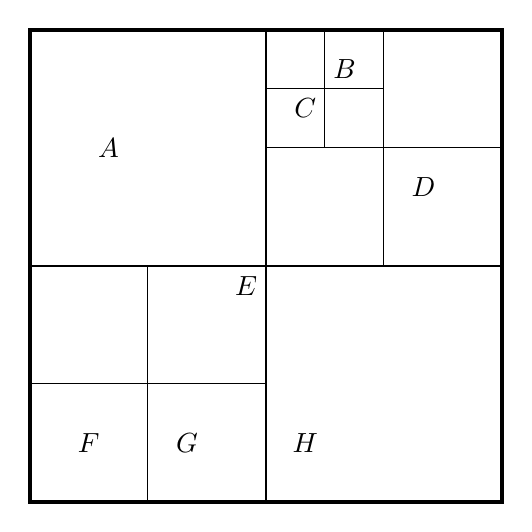
\begin{tikzpicture}[level 1/.style={level distance=1.5cm}]
    % First Layer
    \draw [line width=0.5mm] (0, 0) rectangle (6, 6);

    % Second Layer 
    \draw [line width=0.25mm] (0, 0) rectangle (3, 3);
    \draw [line width=0.25mm] (3, 0) rectangle (6, 3);
    \draw [line width=0.25mm] (0, 3) rectangle (3, 6);
    \draw [line width=0.25mm] (3, 3) rectangle (6, 6);

    % Third Layer (South West)
    \draw [line width=0.125mm] (0, 0) rectangle (1.5, 1.5);
    \draw [line width=0.125mm] (1.5, 1.5) rectangle (3, 3);

    % Third Layer (North East)
    \draw [line width=0.125mm] (3, 3) rectangle (4.5, 4.5);
    \draw [line width=0.125mm] (4.5, 4.5) rectangle (6, 6);

    % Forth Layer (North West)
    \draw [line width=0.125mm] (3, 4.5) rectangle (3.75, 5.25);
    \draw [line width=0.125mm] (3.75, 5.25) rectangle (4.5, 6);

    % Draw the nodes
    \node at (1, 4.5) {$A$};
    \node at (4, 5.5) {$B$};
    \node at (3.5, 5) {$C$};
    \node at (5, 4) {$D$};
    \node at (2.75, 2.75) {$E$};
    \node at (0.75, 0.75) {$F$};
    \node at (2, 0.75) {$G$};
    \node at (3.5, 0.75) {$H$};
\end{tikzpicture}
\end{minipage}
\caption{Unterteilung einer Galaxie in verschiedene Zellen}
\label{fig:cells}
\end{figure}

\begin{figure}
\begin{forest}
    for tree={circle,draw, s sep+=0.25em}
    [
        [A]
        [
            [
                []
                [B]
                [C]
                []
            ]
            []
            []
            [D]
        ]
        [
            []
            [E]
            [F]
            [G]
        ]
        [H]
    ]
\end{forest}
\caption{Die in Abbildung \ref{fig:cells} dargestellte Galaxie als Baum
dargestellt}
\end{figure}

Um die Kraft die auf einen bestimmten Stern wirkt zu berechnen, wird der Baum
von der Wurzel aus nach unten durchlaufen.  Beispiel: Berechnung der Kraft die
auf den Stern A wirkt. Der 'Quadtree' wird von oben nach unten durchgegangen,
also wird das Verhältnis zwischen der Entfernung des Massemittelpunktes zu dem
Stern A (\(\approx 42\)) und der Breite der jeweiligen Zelle (100) berechnet
(Formel \ref{eq:barnes_hut}): \( \frac{100}{43} \not> \theta = 0.5\).

\begin{equation} \label{eq:barnes_hut} \theta = \frac{d}{r} \end{equation}

Ist das Verhältnis größer als ein im vorhinein definierter Grenzwert \( \theta
\), dann wird weiter in den Quadtree ineingegangen und eine Ebene tiefer
rekursiv weitergeprüft.

Hierbei ist es wichtig, dass die Sterne richtig in den Baum eingefügt wurden,
d.h.: Die eigentlichen Sterne müssen in den Blättern liegen. Um dies zu
erreichen, müssen die Sterne beim einfügen immer in der Blätter verschoben
werden.

\begin{figure}
\subfigure[Anfangszustand. Der Stern B soll in den Baum, indem sich bereits A befindet, eingefügt werden.]{
    \begin{forest}
        for tree={circle,draw, s sep+=0.25em}
        [,phantom
            [B]
            [
                A
                []
                []
                []
            ]
        ]
    \end{forest}
}
\quad
\subfigure[Stern B kann nicht eingefügt werden, da der Slot durch A belegt ist, also wird A weiter in den Baum versickert.]{
    \begin{forest}
        for tree={circle,draw, s sep+=0.25em}
        [,phantom
            [B]
            [
                [A
                    []
                    []
                    []
                ]
                []
                []
            ]
        ]
    \end{forest}
}
\quad
\subfigure[B wird nun eingefügt, da sich B jedoch nicht in einem Blatt befinden, muss B weiter versickert werden.]{
    \begin{forest}
        for tree={circle,draw, s sep+=0.25em}
        [,phantom
            [B
                [A
                    []
                    []
                    []
                ]
                []
                []
            ]
        ]
    \end{forest}\quad\\[2ex]
}
\quad
\subfigure[Damit B versickert werden kann, wird der Platz der durch A besetzt wird freigemacht, indem A weiter versickert wird.]{
    \begin{forest}
        for tree={circle,draw, s sep+=0.25em}
         [B
             [
                 [A
                     []
                     []
                     []
                 ]
                 []
                 [
                     []
                     []
                     []
                 ]
             ]
             []
             []
         ]
    \end{forest}\quad
}
\quad
\subfigure[B kann jetzt in den Baum versickert werden und ist nun ein Blatt.]{
    \begin{forest}
        for tree={circle,draw, s sep+=0.25em}
         [
             [
                 [A
                     []
                     []
                     []
                 ]
                 []
                 [B
                     []
                     []
                     []
                 ]
             ]
             []
             []
         ]
    \end{forest}\quad
}

\caption{Schrittweises einfügen des Sternes B in einen Baum, indem sich bereits ein Stern (A) befindet.} \label{fig:insertwithexisting}
\end{figure}

\begin{lstlisting}
if node.hasstar() {

}
\end{lstlisting}

Wie in Abbildung \ref{fig:insertwithexisting} zu sehen ist, wird erst der
bereits existierende Stern weiter in den Baum versickert, der Stern welcher
eingefügt werden soll wird danach ebenfalls in den Baum Versickert bis er sich
in einem der Blätter befindet.

Die Koordinate des Massenmittelpunktes \( \varsigma \) des jeweiligen Knotens
kann wie in Formel (\ref{eq:mean_mass}) beschrieben berechnet werden:

\begin{equation} \label{eq:mean_mass}
\varsigma = \left( \dfrac{ \displaystyle \sum_{i=0}^{n} x_i \cdot m_i }{
\displaystyle \sum_{i=0}^{n} m_i } , \frac{ \displaystyle \sum_{i=0}^{n} y_i
\cdot m_i }{ \displaystyle \sum_{i=0}^{n} m_i } \right)
\end{equation}

Es ist somit durch \( \theta \) eine End Bedingung gegeben, welche verhindert
das zu weit in den Baum vorgedrungen wird und somit auch verhindert, dass
Sterne die in einer zu großen Entfernung zu dem ursprungssten liegen und dicht
genug grupiert sind zusammengefasst werden.

\subsubsection{Implementierung des Quadtrees}
Um generell irgendwas zu tun muss in fast allen fällen etwas definiert werden.
Zur Simulation von Galaxien brauchen wir vor allem eine Methode, Sterne
einheitlich zu definieren. Der unten definierte Vec2-typ kann einen Vektor oder
eine Koordinate darstellen was ihn in der Anwendung zu einem praktischen
Hilfsmittel macht.  Er speichert die X und Y Komponente der jeweiligen Struktur
die er darstellen soll als float64-typ.

\begin{lstlisting}
type Vec struct {
        X               float64
        Y               float64
        Z               float64
}

method (Vec2) insert() {...}
method (Vec2) insideOf() bool {...}
func newVec2() Vec2 {...}
\end{lstlisting}

Mithilfe des Vec2-typens kann ein Kompletter Stern definiert werden. Dabei wird
ein Stern mithilfe seine Position \( C \), seiner Geschwindigkeit \( V \), und
seiner Masse \( M \) beschrieben.

\begin{lstlisting}
type Star struct {
        C               Vec
        V               Vec
        Mass            float64
}

method (Vec2) insideOf() bool {...}
\end{lstlisting}

Um einen sogennanten quadtree bzw. octree aufzubauen wird erstmal eine
Räumliche Begrenzung benötigt, die einem Raum beschriebt indem die Sterne
enthalten sind oder nicht.  Diese grenze ist als `Boundary` definiert, es wird
dabei der Mittelpunkt der Begrenzung und die kürzeste Entfernung zwischen
mittelpunkt und äußerer Begrenzung genutzt um den Raum zu definieren.

\begin{lstlisting}
type Boundary struct {
        Center          Vec
        HalfDimension   float64
}

function newBoundary() {...}
\end{lstlisting}

Der eigentliche QuadTree bzw. Octree beinhaltet einige Informationen: Die
Anzahl in ihm enthaltene Sterne, die Räumliche Ausbereitung, die eigentlichen
Sterne als Star2D definiert und die Rekursionstiefe als integer. Die Definition
des Quadtrees der Unten zu sehen ist enthält Zeiger zu den Kindern des
Quadtrees und ist somit rekursiv definiert was es einfach macht neue Kinder zu
erstellen, da diese eine Kopie ihre Eltern mit einer anderen Begrenzung
darstellen wodurch die in ihnen enthaltenen Sterne weniger werden.

\begin{lstlisting}
type QuadTree struct {
        StarCount       int
        Boundary        Boundary
        Star            []Vec2

        NorthWest       *QuadTree
        NorthEast       *QuadTree
        SouthWest       *QuadTree
        SouthEast       *QuadTree

        ReccursionDepth int
}
method (QuadTree) insert(Star) bool {...}
method (QuadTree) subdivide() {...}
\end{lstlisting}

\subsubsection{Benchmarking}

Um den Geschwindigkeit Vorteil darzustellen, kann die Kraft zwischen \(n\)
homogen verteilten Sternen berechnet werden. Einmal mit der Brute-Force Methode
und einmal mit der im Barnes-Hut Algorithmus beschriebenen Methode.

\subsubsection{Runge-Kutta Methoden}
Die Runge-Kutta Methode wird genutzt, um die Position eines Objektes nach einer
Beliebigen Zeit zu approximieren. Dabei kann, bei Nutzung eines möglich kleinen
Zeit Schrittes, ein sehr genaues Ergebnis erzielt werden.  In unserem Fall
haben wir einen Stern auf den eine Kraft wirkt. Wir wollen die Position des
Sterns nach einem Zeit schritt berechnen, jedoch auch eine andere Kraft mit
einbringen um die Sterne auf eine Elliptische Bahn um die Mitte der Galaxie zu
bringen.  Die Geschwindigkeit die der Stern dabei annimmt kann mit der
folgenden Formel berechnet werden:

\begin{equation}
    v = \sqrt{ar}
\end{equation}

\subsubsection{Goroutines}
Die Nutzung von mehreren sogenannten Go-Methoden ist unglaublich effektiv, da
es die Zeit die gebraucht wird das Programm auszuführen drastisch verringert.
Die Implementation ist ebenfalls unglaublich einfach, es recht

\subsection{Netzwerk}

Damit das Projekt so gut wie möglich skaliert, wird die Anwendung in mehrere
kleine Dienste aufgeteilt die jeweils eine Funktion übernehmen und
untereinander kommunizieren. Dabei läuft jede Anwendung in einem eigenen
Container (siehe \ref{subsubsec:Docker}) und kann somit in falle eines
Nadelöhrs mehrfach gestartet werden und über einen Reverse-http-Proxy (siehe
\ref{subsubsec:Traefik}) mit Daten versorgt werden.

\subsubsection{Die verschiedenen Dienste}
Um die Generierung der Punkt Wolken und die anschließende Simulation der Wolke
in einzelne Micro Services aufzuspalten muss erstmal definiert werden für welche
Dienste es überhaupt Sinn macht sie in einzelne Instanzen abhängig bzw.
unabhängig von einander agieren.

\subsubsection{Docker} \label{subsubsec:Docker}
\begin{quote}
\begin{minipage}{\linewidth}
\stepcounter{footnote}
\renewcommand\thempfootnote{\arabic{footnote}}
``Docker vereinfacht die Bereitstellung von Anwendungen, weil sich Container,
die alle nötigen Pakete enthalten, leicht als Dateien transportieren und
installieren lassen. Container gewährleisten die Trennung und Verwaltung der
auf einem Rechner genutzten Ressourcen. Das beinhaltet laut Aussage der
Entwickler: Code, Laufzeit Modul, System Werkzeuge, Systembibliotheken – alles
was auf einem Rechner installiert werden kann.``~\footnote{\url{https://de.wikipedia.org/wiki/Docker_(Software)}}
\end{minipage}
\end{quote}

\subsubsection{Docker-compose}
Damit nicht alle Container per Hand auf jedem System gestartet werden müssen
wird eine sogenannte Docker-compose Datei erstellt, diese ermöglicht es einem
die komplette Docker Konfiguration in einer Datei zu bündeln und somit auch die
jeweiligen Netzwerke einfacher zu konfigurieren.

\subsubsection{Traefik} \label{subsubsec:Traefik}
\subsubsection{Kubernetes}
\subsubsection{Grafana}

